\documentclass{article}
\usepackage[utf8]{inputenc}
\usepackage{pgfplots}

\title{\HUGE Lab1}
\author{\LARGE Dilip kunderu}
\date{\large September 20 2016}

\begin{document}

\maketitle

\newpage

\section{Access to shared Buffer}
Having a deferential access to shared buffer in an asynchronous fashion,

    \begin{itemize}
        \item Although two processes use the processor, the time required by each of the processes might differ. Thus, a lot of processor cycles get invested in computations which are erroneous.
        \item Buffer might have an overflow/underflow condition if the access is not synchronized, leading again to wasted processor cycles and/or loss of data
        \item Complex computations to be made by data returned by the consumer process will
            \begin{enumerate}
                \item inconsistent state of the data
                \item busy waiting condition 
            \end{enumerate}
    \end{itemize}

\section{Semaphore vs Mutex in lieu of waiting efficiency}
In the case of Mutex implementation
    \begin{itemize}
        \item All processes have the same wait time as the \textbf{entire} buffer is locked when a process acquires the mutex.
        \item Though the uniformity is a plus, median wait time is higher in this implementation.
    \end{itemize}
In the case of the counting semaphore implementation
    \begin{itemize}
        \item In the case of the most usual implementation, consumer initially waits till the buffer is full, and then starts the action.
        \item Unless a boundary condition is defined, an offset amounting to the buffer size would be witnessed in the output log all the time
        \item Though all items produced are consumed in-order, the average wait time for this implementation is higher.
    \end{itemize}
    In short,
    \begin{itemize}
        \item Utilizing \textbf{Mutex} mechanisms locks the usage of the complete buffer down to only one process. In contrast, employing a general \textbf{semaphore} would allow a more granular access to the individual nodes of the buffer/ user-defined division of the buffer memory.
        \item \textbf{Mutex} is more like a \textit{locking} mechanism on the buffer, and a Mutex lock can only be resumed by the process that acquired the lock initially.
        A (counting) \textbf{semaphore}, is slightly different, in the sense that it is more of a \textit{signaling} mechanism, with an important differentiators being that \textit{wait()} and \textit{signal()} can be issued by different processes.
        \item Though both semaphore and mutex mechanisms solve the producer-consumer problem, wait time while deploying a counting semaphore tends to vary, in contrast to a mutex.\\
        While running a counting semaphore, the consumer process waits until the buffer is full, and then start with its output. In a perpetual loop, it will theoretically output all the items, in the order which they are produced, but not necessarily in the form of an \textit{atomic} transaction ie., consuming the data immediately after the producer produces it.\\
        This is the prime difference that I could see between the two implementations.  
    \end{itemize}
    
\section{Timing Plots for the codes}
The following are the timing plots of the codes :

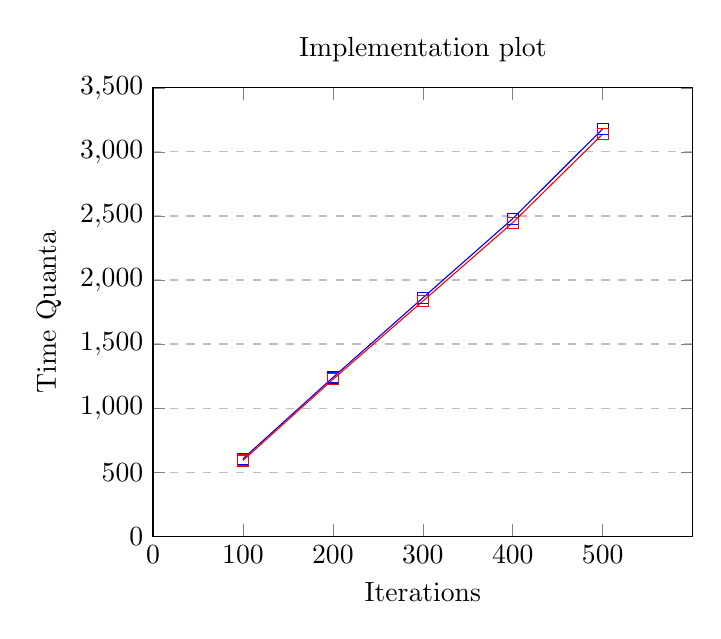
\begin{tikzpicture}
\begin{axis}[
    title={Implementation plot},
    xlabel={Iterations},
    ylabel={Time Quanta},
    xmin=0, xmax=600,
    ymin=0, ymax=3500,
    xtick={0,100,200,300,400,500},
    ytick={0,500,1000,1500,2000,2500,3000,3500},
    ymajorgrids=true,
    grid style=dashed,
]
 
\addplot[
    color=blue,
    mark=square,
    ]
    coordinates {
    (100,604)(200,1239)(300,1860)(400,2479)(500,3180)};
 
 \addplot[
    color=red,
    mark=square,
    ]
    coordinates {
    (100,591)(200,1224)(300,1835)(400,2448)(500,3139)};
\end{axis}
\end{tikzpicture}

The plots seem to overlap because
\begin{itemize}
    \item Only 1 producer and one consumer processes are being run
    \item Iterations are too little to witness variances
\end{itemize}
\end{document}
